% -----------------------------------------------------------------
% Document class: Article
\documentclass[ a4paper, twoside, 11pt]{article}
\usepackage{../../macros-general}
\usepackage{../../macros-article}
% Number of the handout, quiz, exam, etc.
\newcommand{\numero}{01}
\setcounter{numero}{\numero}
\graphicspath{{./figures/}}

% -----------------------------------------------------------------
\begin{document}
\allowdisplaybreaks

% Indices
\newcommand{\iava}{$i$\tsup{ava} }
\newcommand{\iavo}{$i$\tsup{avo} }
\newcommand{\java}{$j$\tsup{ava} }
\newcommand{\javo}{$j$\tsup{avo} }
\newcommand{\kava}{$k$\tsup{ava} }
\newcommand{\kavo}{$k$\tsup{avo} }
\newcommand{\tava}{$t$\tsup{ava} }
\newcommand{\tavo}{$t$\tsup{avo} }
\newcommand{\tmava}{$(t-1)$\tsup{ava} }
\newcommand{\tmavo}{$(t-1)$\tsup{avo} }
\newcommand{\tMava}{$(t+1)$\tsup{ava} }
\newcommand{\tMavo}{$(t+1)$\tsup{avo} }

\begin{center}
\Large Sistemas de Control (EYAG-1005): Tarea \numero \\[1ex]
\small \textbf{Semestre:} 2017-2018 T\'ermino I \qquad
\textbf{Instructor:} Luis I. Reyes Castro
\end{center}
\halfskip

\textbf{Ponderaci\'on:} Cada problema equivale a un punto. 
\fullskip

% -----------------------------------------------------------------
\begin{problem}
En el siguiente sistema mec\'anico la entrada es el torque $T(t)$ y la salida es el desplazamiento del bloque de masa $x(t)$. Encuentre la funci\'on de transferencia, \iec
\[
G(s) \, = \, 
\frac{X(s)}{T(s)}
\]
\begin{figure}[htb]
\centering
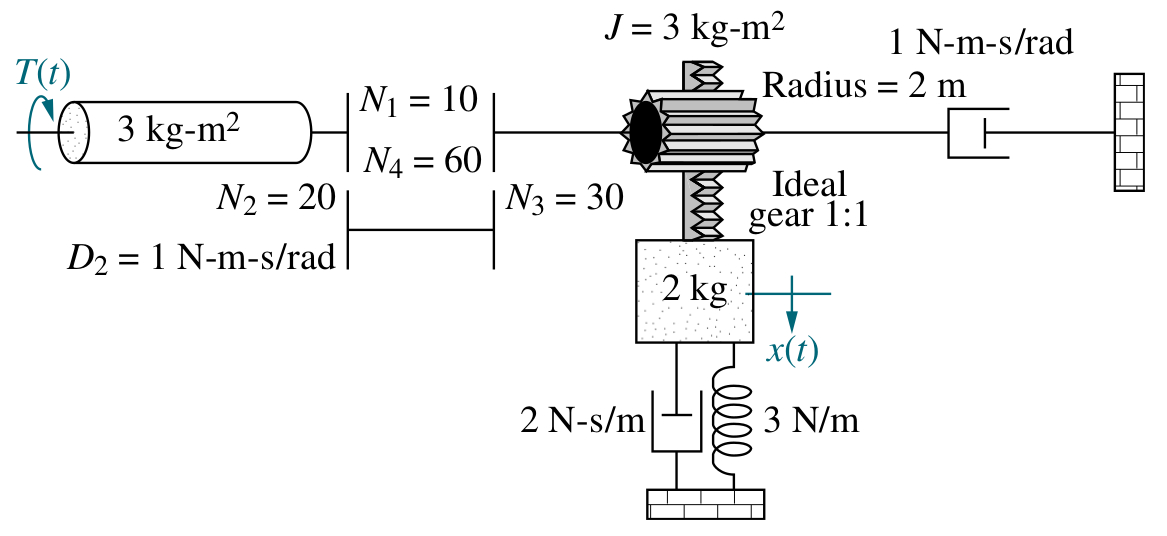
\includegraphics[width=0.68\textwidth]{figures/Nise_Prob-2-40.jpg}
\end{figure}

\end{problem}
\vspace{\baselineskip}

% -----------------------------------------------------------------
\begin{problem}
Considere el siguiente sistema mec\'anico rotacional donde un motor de corriente directa (DC) controlado por armadura sirve de actuador. La entrada es el voltage de la armadura $e_a(t)$ y la salida es el desplazamiento angular $\theta_2(t)$. Encuentre la funci\'on de transferencia, \iec
\[
G(s) \, = \, 
\frac{\Theta_2(s)}{E_a(s)}
\]
\begin{figure}[H]
\centering
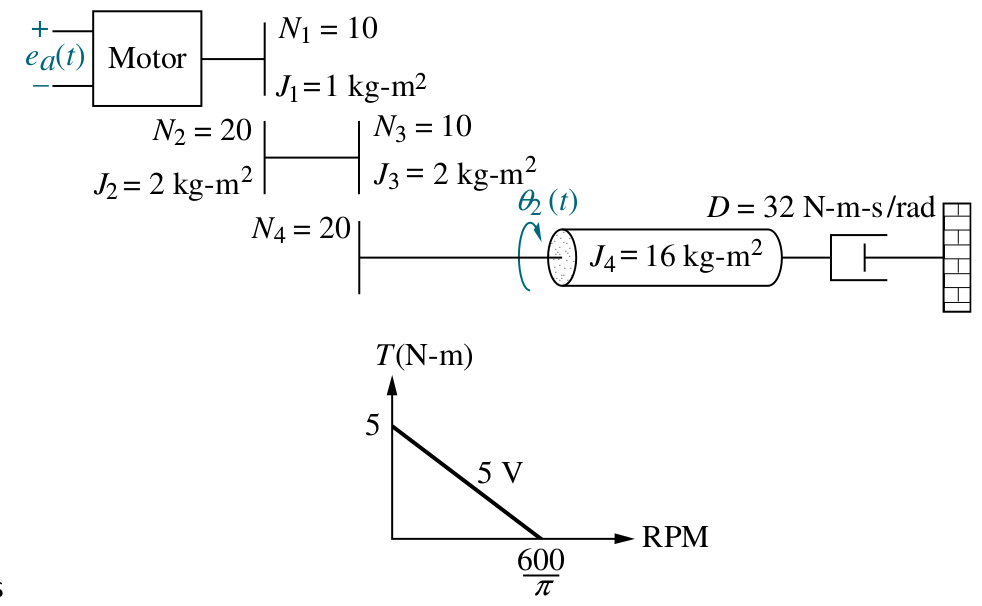
\includegraphics[width=0.66\textwidth]{figures/Nise_Prob-2-43.jpg}
\end{figure}

\end{problem}
\vspace{\baselineskip}

% -----------------------------------------------------------------
\begin{problem}
Un giroscopio es un instrumento para medir velocidades angulares. Considere el siguiente modelo de un giroscopio de un solo grado de libertad que mide velocidades angulares en el eje-$z$ y produce deflecciones angulares en el eje-$x$, cuya ecuaci\'on diferencial es: \[
J_x \, \ddot{\theta}_x(t) + D_x \, \dot{\theta}_x(t) + K_x \, \theta_x(t)
\,  = \, J \, \omega \, \dot{\theta}_z(t)
\]
\fullcut
\fullcut
\begin{figure}[htb]
\centering
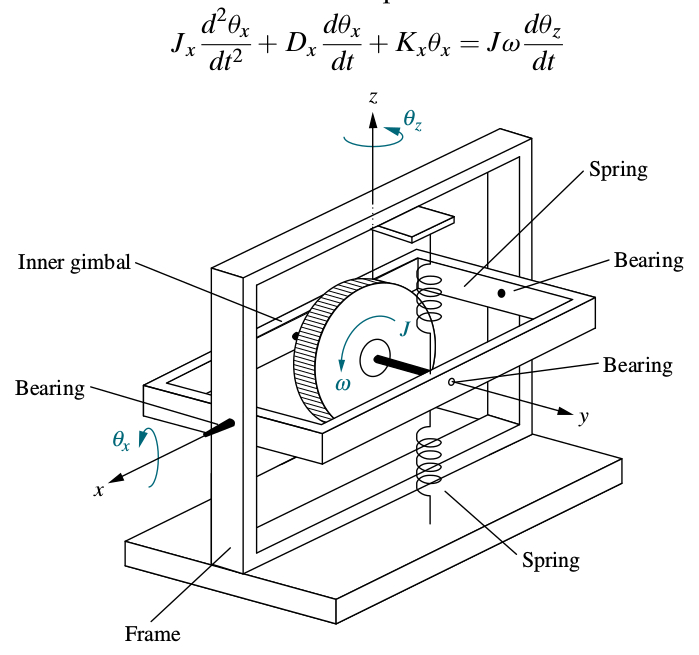
\includegraphics[ width = 0.6\textwidth]{figures/Nise_Prob-3-17.jpg}
\end{figure}

Suponiendo adem\'as que el eje-$x$ est\'a conectado a un potenci\'ometro que indica $c$ voltios por cada grado de deflecci\'on, y denotando al voltage de salida del potenci\'ometro como $v_{pot}(t)$, encuentre la funci\'on de transferencia del giroscopio, \iec
\[
G(s) \, = \, 
\frac{V_{pot}(s)}{\Theta_z(s)}
\]

\end{problem}
\vspace{\baselineskip}

% -----------------------------------------------------------------
\begin{problem}
Para el siguiente sistema de control, encuentre su funci\'on de transferencia en circuito cerrado como funci\'on de $K$. 

\begin{figure}[H]
\centering
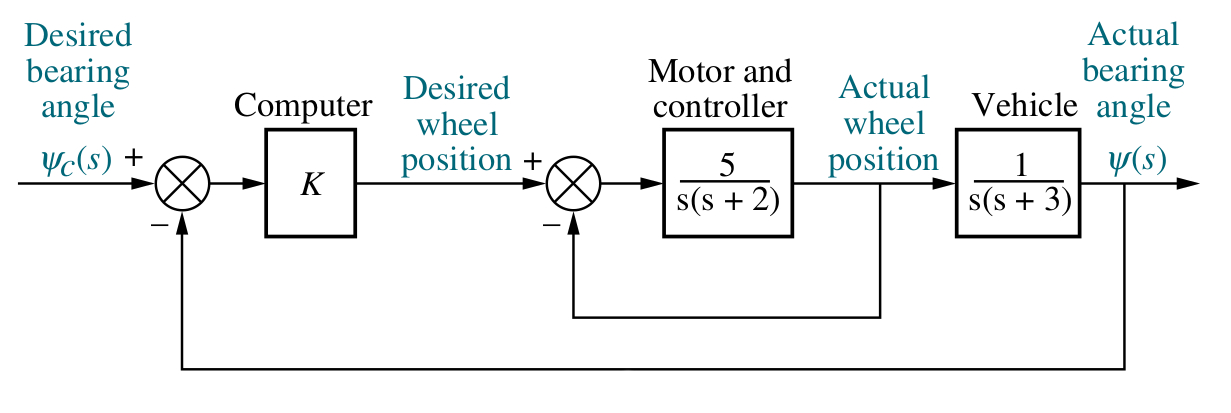
\includegraphics[width=0.74\textwidth]{figures/Nise_Prob-5-51.jpg}
\end{figure}

\end{problem}
\vspace{\baselineskip}

% -----------------------------------------------------------------
\begin{problem}
Considere el sistema de control de posici\'on angular mostrado en la figura de arriba. Con esto en mente: 
\begin{enumerate}[label=\alph*.]
\item Encuentre valores para las ganancias $K_1$ y $K_f$ de tal manera que las m\'etricas de respuesta en el tiempo del sistema en circuito cerrado sean: 
\begin{itemize}
\item Porcentaje de sobrepaso del 25\%. 
\item Tiempo de asentamiento de 0.2 segundos. 
\end{itemize}
\item Calcule el error en estado estable del sistema en circuito cerrado para una entrada escal\'on $r(t) = u(t)$ y para una entrada rampa $r(t) = t \, u(t)$. 
\end{enumerate}

\begin{figure}[H]
\centering
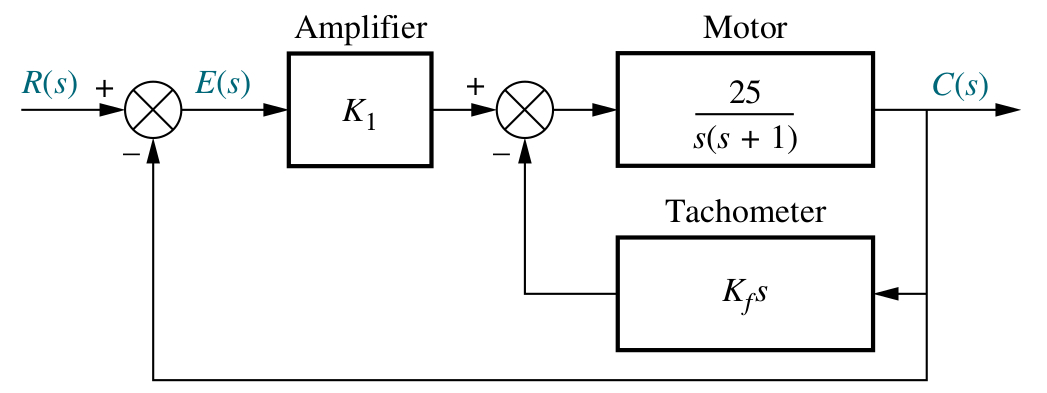
\includegraphics[ width = 0.6\textwidth]{figures/fig_P9-8.jpg}
\end{figure}

\end{problem}
\vspace{\baselineskip}

% -----------------------------------------------------------------
\begin{problem}
Considere el sistema de control de cabeceo de un veh\'iculo a\'ereo no-tripulado mostrado en la figura de abajo. 

\begin{figure}[htb]
\centering
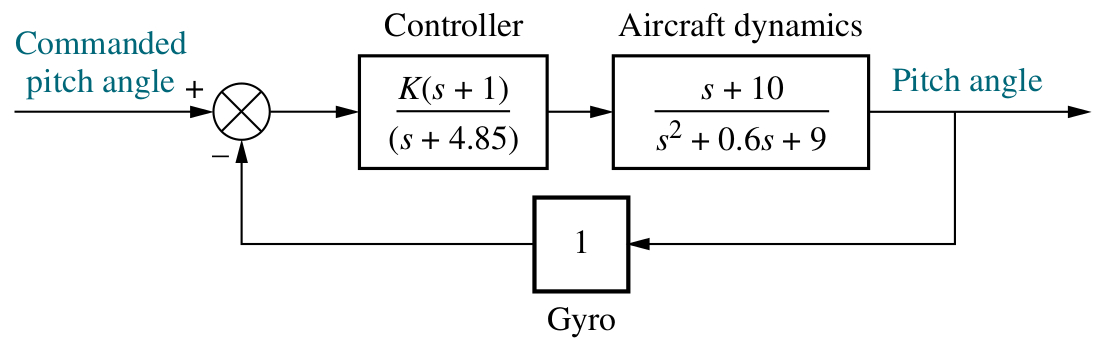
\includegraphics[ width = 0.64\textwidth]{figures/fig_P6-12.jpg}
\end{figure}

Con esto en mente: 
\begin{enumerate}[label=\alph*.]
\item Asumiendo la forma del controlador mostrada en la figura, bosqueje el lugar geom\'etrico de las ra\'ices \emph{(root locus)}. 
\item De acuerdo a su bosquejo anterior, determine la veracidad o falsedad de cada uno de las siguientes proposiciones. 
\begin{itemize}
\item Existe al menos un valor de la ganancia $K$ tal que si $K$ es inferior a ese valor entonces el sistema es estable. 
\item Existe al menos un valor de la ganancia $K$ tal que si $K$ es superior a ese valor entonces el sistema es inestable.  
\item Existe un valor de la ganancia $K$ para el cual todos los polos son complejos. 
\item Existe un valor de la ganancia $K$ para el cual todos los polos son reales. 
\end{itemize}

\end{enumerate}

\end{problem}
\vspace{\baselineskip}

\end{document}
